\chapter{Hệ phương trình Maxwell và sóng điện từ}
\begin{vd}[Cáp đồng trục và tích điện bề mặt]
 Một cáp đồng trục rất dài bao gồm lõi trụ bên trong có bán kính $a$ và độ dẫn điện đẳng hướng $\sigma$, được bọc bởi một lớp vỏ mỏng bên ngoài có bán kính $b$. Lớp vỏ bọc có độ dẫn điện bằng vô cùng. Khoảng trống giữa lớp vỏ và lõi trụ là chân không. Một dòng điện có mật độ dòng đều $J$, hướng theo trục tọa độ $z$, được cho chạy qua lõi trụ bên trong. Dòng điện chạy ngược lại cũng được phân bố đều trên lớp vỏ bên ngoài (như hình vẽ). Tính mật độ điện mặt của điện tích trên bề mặt của lõi trụ trong như một hàm của tọa độ $z$, với gốc tọa độ $z=0$ được chọn tại chính giữa cáp (cách đều hai đầu cáp).
         %đính hình vẽ
         \begin{center}


\tikzset{every picture/.style={line width=0.75pt}} %set default line width to 0.75pt        

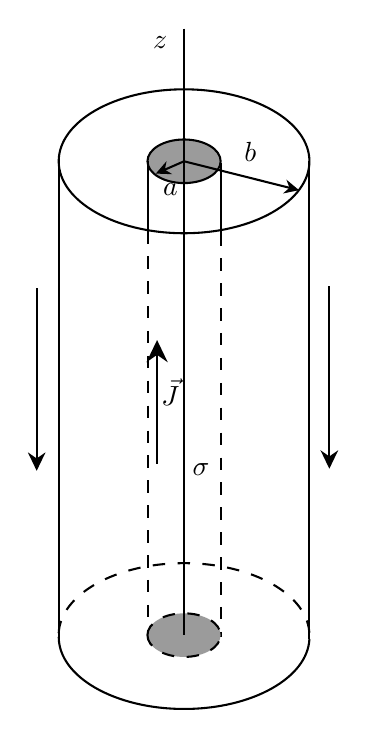
\begin{tikzpicture}[x=0.75pt,y=0.75pt,yscale=-1,xscale=1]
%uncomment if require: \path (0,506); %set diagram left start at 0, and has height of 506

%Shape: Ellipse [id:dp08514119741879456] 
\draw   (220,146.07) .. controls (220,126.92) and (247.04,111.4) .. (280.4,111.4) .. controls (313.76,111.4) and (340.8,126.92) .. (340.8,146.07) .. controls (340.8,165.22) and (313.76,180.74) .. (280.4,180.74) .. controls (247.04,180.74) and (220,165.22) .. (220,146.07) -- cycle ;
%Straight Lines [id:da6580345349354657] 
\draw    (220,146.07) -- (220,376.2) ;
%Straight Lines [id:da7576243264135754] 
\draw    (340.8,146.07) -- (340.8,376.2) ;
%Shape: Arc [id:dp5499873036980762] 
\draw  [draw opacity=0][dash pattern={on 4.5pt off 4.5pt}] (220,373.44) .. controls (220.85,354.72) and (247.56,339.7) .. (280.38,339.7) .. controls (313.73,339.7) and (340.78,355.22) .. (340.78,374.37) .. controls (340.78,374.4) and (340.77,374.42) .. (340.77,374.44) -- (280.38,374.37) -- cycle ; \draw  [dash pattern={on 4.5pt off 4.5pt}] (220,373.44) .. controls (220.85,354.72) and (247.56,339.7) .. (280.38,339.7) .. controls (313.73,339.7) and (340.78,355.22) .. (340.78,374.37) .. controls (340.78,374.4) and (340.77,374.42) .. (340.77,374.44) ;
%Shape: Arc [id:dp5688502623676199] 
\draw  [draw opacity=0] (340.8,376.2) .. controls (339.94,394.92) and (313.24,409.94) .. (280.42,409.94) .. controls (247.06,409.94) and (220.02,394.42) .. (220.02,375.27) .. controls (220.02,375.25) and (220.02,375.22) .. (220.02,375.2) -- (280.42,375.27) -- cycle ; \draw   (340.8,376.2) .. controls (339.94,394.92) and (313.24,409.94) .. (280.42,409.94) .. controls (247.06,409.94) and (220.02,394.42) .. (220.02,375.27) .. controls (220.02,375.25) and (220.02,375.22) .. (220.02,375.2) ;
%Straight Lines [id:da6703551667591763] 
\draw  [dash pattern={on 4.5pt off 4.5pt}]  (262.9,179.8)-- (262.9,375.83) ;
%Straight Lines [id:da26248937521963756] 
\draw  [dash pattern={on 4.5pt off 4.5pt}]  (297.98,180.8)-- (297.98,375.15) ;
%Shape: Ellipse [id:dp2949382826618787] 
\draw  [fill={rgb, 255:red, 155; green, 155; blue, 155 }  ,fill opacity=1 ] (262.77,146.07) .. controls (262.77,140.27) and (270.66,135.57) .. (280.4,135.57) .. controls (290.14,135.57) and (298.03,140.27) .. (298.03,146.07) .. controls (298.03,151.87) and (290.14,156.57) .. (280.4,156.57) .. controls (270.66,156.57) and (262.77,151.87) .. (262.77,146.07) -- cycle ;
%Straight Lines [id:da9075219486272503] 
\draw    (262.9,146.07) -- (262.9,179.8);
%Straight Lines [id:da457304577699581] 
\draw    (297.98,147.07) -- (297.98,180.8);
%Shape: Ellipse [id:dp015579774393628343] 
\draw  [fill={rgb, 255:red, 155; green, 155; blue, 155 }  ,fill opacity=1 ][dash pattern={on 4.5pt off 4.5pt}] (262.75,374.37) .. controls (262.75,368.57) and (270.64,363.87) .. (280.38,363.87) .. controls (290.11,363.87) and (298,368.57) .. (298,374.37) .. controls (298,380.17) and (290.11,384.87) .. (280.38,384.87) .. controls (270.64,384.87) and (262.75,380.17) .. (262.75,374.37) -- cycle ;
%Straight Lines [id:da3177532142519628] 
\draw    (280.38,82.2) -- (280.38,374.37) ;
%Straight Lines [id:da5637404634402237] 
\draw    (269.55,150.8)-- (280.4,146.07) ;
\draw [shift={(266.8,152)}, rotate = 336.44] [fill={rgb, 255:red, 0; green, 0; blue, 0 }  ][line width=0.08]  [draw opacity=0] (7.14,-3.43) -- (0,0) -- (7.14,3.43) -- (4.74,0) -- cycle    ;
%Straight Lines [id:da5165242278954159] 
\draw    (332.89,159.27) -- (280.4,146.07) ;
\draw [shift={(335.8,160)}, rotate = 194.11] [fill={rgb, 255:red, 0; green, 0; blue, 0 }  ][line width=0.08]  [draw opacity=0] (7.14,-3.43) -- (0,0) -- (7.14,3.43) -- (4.74,0) -- cycle    ;
%Straight Lines [id:da1992813532410005] 
\draw    (267.4,235.2) -- (267.4,292.07) ;
\draw [shift={(267.4,232.2)}, rotate = 90] [fill={rgb, 255:red, 0; green, 0; blue, 0 }  ][line width=0.08]  [draw opacity=0] (10.72,-5.15) -- (0,0) -- (10.72,5.15) -- (7.12,0) -- cycle    ;
%Straight Lines [id:da02921768290321003] 
\draw    (209.4,207.2) -- (209.4,292.2) ;
\draw [shift={(209.4,295.2)}, rotate = 270] [fill={rgb, 255:red, 0; green, 0; blue, 0 }  ][line width=0.08]  [draw opacity=0] (8.93,-4.29) -- (0,0) -- (8.93,4.29) -- (5.93,0) -- cycle    ;
%Straight Lines [id:da9014363078063687] 
\draw    (350.4,206.2) -- (350.4,291.2) ;
\draw [shift={(350.4,294.2)}, rotate = 270] [fill={rgb, 255:red, 0; green, 0; blue, 0 }  ][line width=0.08]  [draw opacity=0] (8.93,-4.29) -- (0,0) -- (8.93,4.29) -- (5.93,0) -- cycle    ;


% Text Node
\draw (264,84.4) node [anchor=north west][inner sep=0.75pt]    {$z$};
% Text Node
\draw (268,249.4) node [anchor=north west][inner sep=0.75pt]    {$\vec{J}$};
% Text Node
\draw (268.8,155.4) node [anchor=north west][inner sep=0.75pt]    {$a$};
% Text Node
\draw (308,135.4) node [anchor=north west][inner sep=0.75pt]    {$b$};
% Text Node
\draw (283,290.4) node [anchor=north west][inner sep=0.75pt]    {$\sigma $};


\end{tikzpicture}
\end{center}
\end{vd}
\begin{loigiai}\[\]
Chúng ta viết phương trình Laplace cho vùng không gian giữa hai hình trụ trong hệ tọa độ trụ:
   $$\nabla^{2} \phi=\frac{1}{\rho} \frac{\partial}{\partial \rho}\left(\rho \frac{\partial \phi}{\partial \rho}\right)+\frac{1}{\rho^{2}} \frac{\partial^{2} \phi}{\partial \varphi^{2}}+\frac{\partial^{2} \phi}{\partial z^{2}}=0.$$
Vì tính đối xứng của hệ tọa độ trụ, $\phi$ không phụ thuộc vào $\varphi$ (xem hình vẽ), nên ta có
          \begin{center}
\tikzset{every picture/.style={line width=0.75pt}} %set default line width to 0.75pt        

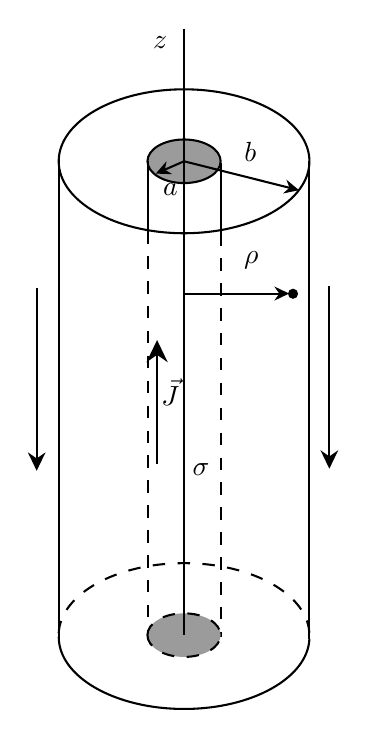
\begin{tikzpicture}[x=0.75pt,y=0.75pt,yscale=-1,xscale=1]
%uncomment if require: \path (0,506); %set diagram left start at 0, and has height of 506

%Shape: Ellipse [id:dp1860886299822715] 
\draw   (220,146.07) .. controls (220,126.92) and (247.04,111.4) .. (280.4,111.4) .. controls (313.76,111.4) and (340.8,126.92) .. (340.8,146.07) .. controls (340.8,165.22) and (313.76,180.74) .. (280.4,180.74) .. controls (247.04,180.74) and (220,165.22) .. (220,146.07) -- cycle ;
%Straight Lines [id:da9188894844845499] 
\draw    (220,146.07) -- (220,376.2) ;
%Straight Lines [id:da30509406818067286] 
\draw    (340.8,146.07) -- (340.8,376.2) ;
%Shape: Arc [id:dp949073474768471] 
\draw  [draw opacity=0][dash pattern={on 4.5pt off 4.5pt}] (220,373.44) .. controls (220.85,354.72) and (247.56,339.7) .. (280.38,339.7) .. controls (313.73,339.7) and (340.78,355.22) .. (340.78,374.37) .. controls (340.78,374.4) and (340.77,374.42) .. (340.77,374.44) -- (280.38,374.37) -- cycle ; \draw  [dash pattern={on 4.5pt off 4.5pt}] (220,373.44) .. controls (220.85,354.72) and (247.56,339.7) .. (280.38,339.7) .. controls (313.73,339.7) and (340.78,355.22) .. (340.78,374.37) .. controls (340.78,374.4) and (340.77,374.42) .. (340.77,374.44) ;
%Shape: Arc [id:dp3443294636844614] 
\draw  [draw opacity=0] (340.8,376.2) .. controls (339.94,394.92) and (313.24,409.94) .. (280.42,409.94) .. controls (247.06,409.94) and (220.02,394.42) .. (220.02,375.27) .. controls (220.02,375.25) and (220.02,375.22) .. (220.02,375.2) -- (280.42,375.27) -- cycle ; \draw   (340.8,376.2) .. controls (339.94,394.92) and (313.24,409.94) .. (280.42,409.94) .. controls (247.06,409.94) and (220.02,394.42) .. (220.02,375.27) .. controls (220.02,375.25) and (220.02,375.22) .. (220.02,375.2) ;
%Straight Lines [id:da18517762688153327] 
\draw  [dash pattern={on 4.5pt off 4.5pt}]  (262.9,179.8) -- (262.9,375.83) ;
%Straight Lines [id:da5108690213132867] 
\draw  [dash pattern={on 4.5pt off 4.5pt}]  (297.98,180.8) -- (297.98,375.15) ;
%Shape: Ellipse [id:dp45650504224312005] 
\draw  [fill={rgb, 255:red, 155; green, 155; blue, 155 }  ,fill opacity=1 ] (262.77,146.07) .. controls (262.77,140.27) and (270.66,135.57) .. (280.4,135.57) .. controls (290.14,135.57) and (298.03,140.27) .. (298.03,146.07) .. controls (298.03,151.87) and (290.14,156.57) .. (280.4,156.57) .. controls (270.66,156.57) and (262.77,151.87) .. (262.77,146.07) -- cycle ;
%Straight Lines [id:da22974417208243958] 
\draw    (262.9,146.07) -- (262.9,179.8) ;
%Straight Lines [id:da21174031134020632] 
\draw    (297.98,147.07) -- (297.98,180.8) ;
%Shape: Ellipse [id:dp02196121657352279] 
\draw  [fill={rgb, 255:red, 155; green, 155; blue, 155 }  ,fill opacity=1 ][dash pattern={on 4.5pt off 4.5pt}] (262.75,374.37) .. controls (262.75,368.57) and (270.64,363.87) .. (280.38,363.87) .. controls (290.11,363.87) and (298,368.57) .. (298,374.37) .. controls (298,380.17) and (290.11,384.87) .. (280.38,384.87) .. controls (270.64,384.87) and (262.75,380.17) .. (262.75,374.37) -- cycle ;
%Straight Lines [id:da009018086778775913] 
\draw    (280.38,82.2) -- (280.38,374.37) ;
%Straight Lines [id:da953359240606179] 
\draw    (269.55,150.8) -- (280.4,146.07) ;
\draw [shift={(266.8,152)}, rotate = 336.44] [fill={rgb, 255:red, 0; green, 0; blue, 0 }  ][line width=0.08]  [draw opacity=0] (7.14,-3.43) -- (0,0) -- (7.14,3.43) -- (4.74,0) -- cycle    ;
%Straight Lines [id:da6169578338464297] 
\draw    (332.89,159.27) -- (280.4,146.07) ;
\draw [shift={(335.8,160)}, rotate = 194.11] [fill={rgb, 255:red, 0; green, 0; blue, 0 }  ][line width=0.08]  [draw opacity=0] (7.14,-3.43) -- (0,0) -- (7.14,3.43) -- (4.74,0) -- cycle    ;
%Straight Lines [id:da6452628135747207] 
\draw    (267.4,235.2) -- (267.4,292.07) ;
\draw [shift={(267.4,232.2)}, rotate = 90] [fill={rgb, 255:red, 0; green, 0; blue, 0 }  ][line width=0.08]  [draw opacity=0] (10.72,-5.15) -- (0,0) -- (10.72,5.15) -- (7.12,0) -- cycle    ;
%Straight Lines [id:da726610125442676] 
\draw    (209.4,207.2) -- (209.4,292.2) ;
\draw [shift={(209.4,295.2)}, rotate = 270] [fill={rgb, 255:red, 0; green, 0; blue, 0 }  ][line width=0.08]  [draw opacity=0] (8.93,-4.29) -- (0,0) -- (8.93,4.29) -- (5.93,0) -- cycle    ;
%Straight Lines [id:da867842048883209] 
\draw    (350.4,206.2) -- (350.4,291.2) ;
\draw [shift={(350.4,294.2)}, rotate = 270] [fill={rgb, 255:red, 0; green, 0; blue, 0 }  ][line width=0.08]  [draw opacity=0] (8.93,-4.29) -- (0,0) -- (8.93,4.29) -- (5.93,0) -- cycle    ;
%Shape: Circle [id:dp6272731743469049] 
\draw  [fill={rgb, 255:red, 0; green, 0; blue, 0 }  ,fill opacity=1 ] (331,209.9) .. controls (331,208.85) and (331.85,208) .. (332.9,208) .. controls (333.95,208) and (334.8,208.85) .. (334.8,209.9) .. controls (334.8,210.95) and (333.95,211.8) .. (332.9,211.8) .. controls (331.85,211.8) and (331,210.95) .. (331,209.9) -- cycle ;
%Straight Lines [id:da08580916155498852] 
\draw    (280.8,209.8) -- (328,209.8) ;
\draw [shift={(331,209.8)}, rotate = 180] [fill={rgb, 255:red, 0; green, 0; blue, 0 }  ][line width=0.08]  [draw opacity=0] (7.14,-3.43) -- (0,0) -- (7.14,3.43) -- (4.74,0) -- cycle    ;


% Text Node
\draw (264,84.4) node [anchor=north west][inner sep=0.75pt]    {$z$};
% Text Node
\draw (268,249.4) node [anchor=north west][inner sep=0.75pt]    {$\vec{J}$};
% Text Node
\draw (268.8,155.4) node [anchor=north west][inner sep=0.75pt]    {$a$};
% Text Node
\draw (308,135.4) node [anchor=north west][inner sep=0.75pt]    {$b$};
% Text Node
\draw (283,290.4) node [anchor=north west][inner sep=0.75pt]    {$\sigma $};
% Text Node
\draw (307.9,188.2) node [anchor=north west][inner sep=0.75pt]    {$\rho $};

\end{tikzpicture}
\end{center}
 
Dạng rút gọn của phương trình Laplace:
     $$\nabla^{2} \phi=\dfrac{1}{\rho} \dfrac{\partial}{\partial \rho}\left(\rho \dfrac{\partial \phi}{\partial \rho}\right)+\dfrac{\partial^{2} \phi}{\partial z^{2}}=0.$$
Như thông thường, chúng ta đặt nghiệm ở dạng:
     $$\phi(\rho,z) = R(\rho)Z(z).$$
và phương trình Laplace bây giờ được biến đổi thành:
   $$\dfrac{1}{R} \dfrac{1}{\rho} \dfrac{\partial}{\partial \rho} \left(\rho \dfrac{\partial R}{\partial \rho}\right) + \dfrac{1}{Z} \dfrac{\partial^2Z}{\partial z^2} = 0.$$
Ta rút gọn phương trình thành:
    $$\dfrac{\partial^2 Z}{\partial z^2} - k^2Z = 0,$$
ở đây $k$ là một hằng số. Bằng cách tịnh tiến đối xứng dọc theo trục $z$,
  $$\dfrac{\partial E_z}{\partial z} = 0 = \dfrac{\partial^2 Z}{\partial z^2}$$
do đó $k=0$, và :
  $$Z(z) = \alpha z + \beta,$$
trong đó $\alpha$ và $\beta$ là hằng số. Thành phần theo phương bán kính bây giờ trở thành:
 $$\dfrac{\partial}{\partial\rho} \left(\rho\dfrac{\partial R}{\partial\rho}\right) = 0$$
 $$R(\rho) = A\ln(\rho/\rho_0).$$
 
Do đó:
   $$\phi(\rho,z) = (\alpha z + \beta)A\ln(\rho/\rho_0).$$
Sử dụng điều kiện biên $(\rho,0) = 0$ dẫn tới $\beta = 0$, và ta có:
   $$\phi(\rho,z) = \tilde{A}z\ln(\rho/\rho_0),$$
trong đó $\tilde{A}$ là một hằng số $(\tilde{A} = \alpha A)$. Chúng ta có thể viết chênh lệch hiệu điện thế dọc trục dưới dạng:
 $$\phi(a,z) - \phi(a,0) = \ot{E}\cdot \ot{z} = \dfrac{Jz}{\sigma}$$
 $$\phi(b,z) - \phi(b,0) = 0,$$
ở dây ta kí hiệu $\ot{J} = \sigma\ot{E}$, là mối liên hệ của mật độ dòng điện $\ot{J}$ và độ dẫn điện đẳng hướng. Ta rút ra:
  $$\tilde{A} z \ln(b/\rho_0) = 0$$
   $$\tilde{A} z \ln(a/\rho_0) = \dfrac{Jz}{\sigma}.$$
Từ đó ta tìm ra :
   $$\rho_0 = b$$
   $$ \tilde{A} = \dfrac{J}{\sigma \ln(a/b)}.$$
Với $\rho < a$, điện thế là tương tự ở trên lớp vỏ, từ đó:
   $$\phi(\rho, z)=\left\{
   \begin{aligned}
\dfrac{J z \ln (\rho / b)}{\sigma \ln (a / b)} ,~ a \leq \rho \leq b \\
\dfrac{J z}{\sigma} ,~ \rho \leq a
\end{aligned}\right. .$$
Mật độ điện mặt là:
  $$\begin{array}{c}
\sigma=\dfrac{E_{\rho}\left(a^{+}\right)-E_{\rho}\left(a^{-}\right)}{4 \pi} \\
\\=\dfrac{1}{4 \pi}\left(-\left.\dfrac{\partial \phi_{a^{+}}}{\partial \rho}\right|_{\rho=a^{+}}+\left.\dfrac{\partial \phi_{a}-}{\partial \rho}\right|_{\rho=a^{-}}\right)=-\dfrac{J z}{4 \pi a \sigma \ln (a / b)},
\end{array}$$
ở đây $a^+$ và $a^-$ lần lượt kí hiệu các điểm bên ngoài và bên trong hình trụ nhỏ.


\end{loigiai}


\begin{vd}[Hộp kín và lực đẩy điện từ]

Hai mặt đối diện nhau của một hộp cứng được tích điện đều với mật độ điện mặt lần lượt là $\sigma$ và $-\sigma$. Mặt tích điện dương được đặt ở vùng $0\leq x \leq a, 0 \leq y \leq b$ của mặt phẳng $z = h$, trong khi đó mặt tích điện âm nằm ở vùng $0\leq x \leq a, 0 \leq y \leq b$ ở mặt phẳng $x$-$y$. Bên trong hộp là một từ trường đều $\ot{B} = (0,B_0,0)$. Giả sử rằng $h$ rất nhỏ so với cả $a$ và $b$ và bề mặt được tích điện không dẫn điện (xem hình vẽ).
  \begin{center}
\tikzset{every picture/.style={line width=0.75pt}} %set default line width to 0.75pt        

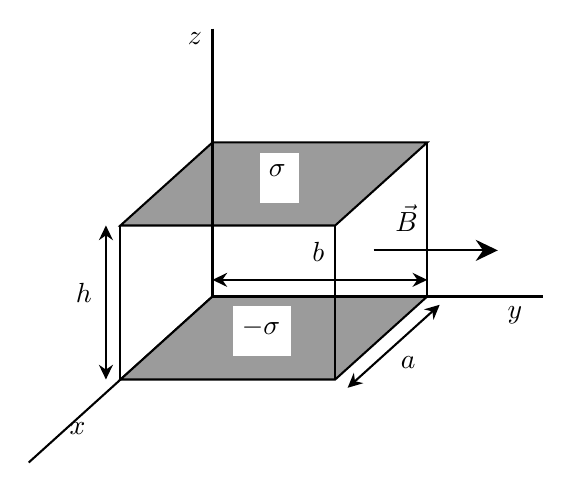
\begin{tikzpicture}[x=0.75pt,y=0.75pt,yscale=-1,xscale=1]
%uncomment if require: \path (0,480); %set diagram left start at 0, and has height of 480

%Shape: Parallelogram [id:dp7383941544633257] 
\draw  [fill={rgb, 255:red, 155; green, 155; blue, 155 }  ,fill opacity=1 ] (231.34,162) -- (334.8,162) -- (290.46,202) -- (187,202) -- cycle ;
%Straight Lines [id:da4225131997996052] 
\draw    (231.34,107.2) -- (231.34,236.2) ;
%Straight Lines [id:da7301010395335319] 
\draw    (142.8,316.2) -- (231.34,236.2) ;
%Shape: Parallelogram [id:dp7659903852503229] 
\draw  [fill={rgb, 255:red, 155; green, 155; blue, 155 }  ,fill opacity=1 ] (231.34,236.2) -- (334.8,236.2) -- (290.46,276.2) -- (187,276.2) -- cycle ;
%Straight Lines [id:da044188315863318284] 
\draw    (231.34,236.2) -- (390.8,236.2) ;
%Straight Lines [id:da35869164231427164] 
\draw    (187,202) -- (187,276.2) ;
%Straight Lines [id:da2470738216594075] 
\draw    (290.46,202) -- (290.46,276.2) ;
%Straight Lines [id:da5438167972691617] 
\draw    (334.8,162) -- (334.8,236.2) ;
%Straight Lines [id:da6584378615817821] 
\draw    (180,205) -- (180,273.2) ;
\draw [shift={(180,276.2)}, rotate = 270] [fill={rgb, 255:red, 0; green, 0; blue, 0 }  ][line width=0.08]  [draw opacity=0] (7.14,-3.43) -- (0,0) -- (7.14,3.43) -- (4.74,0) -- cycle    ;
\draw [shift={(180,202)}, rotate = 90] [fill={rgb, 255:red, 0; green, 0; blue, 0 }  ][line width=0.08]  [draw opacity=0] (7.14,-3.43) -- (0,0) -- (7.14,3.43) -- (4.74,0) -- cycle    ;
%Straight Lines [id:da6988747796596413] 
\draw    (298.69,278.19) -- (338.57,242.21) ;
\draw [shift={(340.8,240.2)}, rotate = 497.95] [fill={rgb, 255:red, 0; green, 0; blue, 0 }  ][line width=0.08]  [draw opacity=0] (7.14,-3.43) -- (0,0) -- (7.14,3.43) -- (4.74,0) -- cycle    ;
\draw [shift={(296.46,280.2)}, rotate = 317.95] [fill={rgb, 255:red, 0; green, 0; blue, 0 }  ][line width=0.08]  [draw opacity=0] (7.14,-3.43) -- (0,0) -- (7.14,3.43) -- (4.74,0) -- cycle    ;
%Straight Lines [id:da8737021413633921] 
\draw    (234.34,228.2) -- (331.8,228.2) ;
\draw [shift={(334.8,228.2)}, rotate = 180] [fill={rgb, 255:red, 0; green, 0; blue, 0 }  ][line width=0.08]  [draw opacity=0] (7.14,-3.43) -- (0,0) -- (7.14,3.43) -- (4.74,0) -- cycle    ;
\draw [shift={(231.34,228.2)}, rotate = 0] [fill={rgb, 255:red, 0; green, 0; blue, 0 }  ][line width=0.08]  [draw opacity=0] (7.14,-3.43) -- (0,0) -- (7.14,3.43) -- (4.74,0) -- cycle    ;
%Straight Lines [id:da8351953889012924] 
\draw    (309,214) -- (365.8,214) ;
\draw [shift={(368.8,214)}, rotate = 180] [fill={rgb, 255:red, 0; green, 0; blue, 0 }  ][line width=0.08]  [draw opacity=0] (10.72,-5.15) -- (0,0) -- (10.72,5.15) -- (7.12,0) -- cycle    ;


% Text Node
\draw  [draw opacity=0][fill={rgb, 255:red, 255; green, 255; blue, 255 }  ,fill opacity=1 ]  (254,167) -- (273,167) -- (273,191) -- (254,191) -- cycle  ;
\draw (257,171.4) node [anchor=north west][inner sep=0.75pt]    {$\sigma $};
% Text Node
\draw  [draw opacity=0][fill={rgb, 255:red, 255; green, 255; blue, 255 }  ,fill opacity=1 ]  (241,241) -- (269,241) -- (269,265) -- (241,265) -- cycle  ;
\draw (244,245.4) node [anchor=north west][inner sep=0.75pt]    {$-\sigma $};
% Text Node
\draw (218,107.4) node [anchor=north west][inner sep=0.75pt]    {$z$};
% Text Node
\draw (161,295.4) node [anchor=north west][inner sep=0.75pt]    {$x$};
% Text Node
\draw (372,239.4) node [anchor=north west][inner sep=0.75pt]    {$y$};
% Text Node
\draw (164,228.4) node [anchor=north west][inner sep=0.75pt]    {$h$};
% Text Node
\draw (320.63,263.6) node [anchor=north west][inner sep=0.75pt]    {$a$};
% Text Node
\draw (278,208.4) node [anchor=north west][inner sep=0.75pt]    {$b$};
% Text Node
\draw (318,190.4) node [anchor=north west][inner sep=0.75pt]    {$\vec{B}$};

\end{tikzpicture}
\end{center}
\begin{enumerate}[1)]
    \item Tính xung lực tác dụng lên hộp khi từ trường bị tắt đi.
    \item Chứng minh rằng xung lực đó chính bằng động lượng của trường điện từ ban đầu.
\end{enumerate}

\end{vd}
\begin{loigiai}
  \begin{enumerate}[1)]
   \item Từ phương trình Maxwell 
   $$\nabla \times \ot{E} = - \frac{1}{c} \frac{\partial B}{\partial t},$$
ta có thể tính được điện trường ở trong hộp. Ta có các thành phần theo phương $\hat{{x}}, \hat{y}$ và ${\hat{z}}$ của phương trình là:
\begin{align*}
    {\hat{x}} \left(\frac{\partial E_z}{\partial y} - \frac{\partial E_y}{\partial z}\right) &= 0,\\
    {\hat{z}} \left(\frac{\partial E_y}{\partial x} - \frac{\partial E_x}{\partial y}\right) &= 0,\\
    -{\hat{y}} \left(\frac{\partial E_z}{\partial x} - \frac{\partial E_x}{\partial z}\right) &= - \frac{1}{c} \frac{\partial B}{\partial t} {\hat{y}}.
\end{align*}
Từ các phương trình đó ta thu được:
\begin{align*}
    E_y &= E_z =0,\\
    E_x &= -\frac{1}{c} \frac{\partial B}{\partial t} z + E_0.
\end{align*}
ở đây $E_0$ là một hằng số. Và từ phương trình lực:

   $$\frac{\dd \ot{P}}{\dd t}=\left(-\left.\sigma a b E_{x}\right|_{z=0}+\left.\sigma a b E_{x}\right|_{z=h}\right) \hat{{x}}=\sigma a b h\left(-\frac{1}{c} \frac{\partial B}{\partial t}\right) \hat{{x}}$$
chúng ta tìm được xung lực tác dụng vào hộp khi từ trường bị tắt đi:
   $$\ot{P}=\sigma a b h \int_{0}^{t}-\frac{1}{c} \frac{\partial B}{\partial t^{\prime}} \dd t^{\prime} \hat{{x}}=\frac{1}{c} \sigma \, a b h B_{0} \hat{{x}}.$$
\item  Động lượng ban đầu có thể tính được từ vector Poynting: 
   $$\ot{S}=\frac{c}{4 \pi}[\ot{E} \times \ot{H}]=\frac{c}{4 \pi}\left|\begin{array}{ccc}
\hat{{x}} & \hat{{y}} & \hat{{z}} \\
0 & 0 & -4 \pi \sigma \\
0 & B_{0} & 0
\end{array}\right|=c \sigma B_{0} \hat{{x}}$$
        $$\ot{P} = \int_{V} \frac{\ot{S}}{c^2}\dd V = \frac{1}{c} \sigma a b h B_0 {\hat{x}} ,$$
kết quả này là giống với kết quả ta thu được từ câu $1).$
\end{enumerate}
\end{loigiai}


\begin{vd}[Liên lạc vô tuyến - Hiệu ứng Hall]
\begin{center}
    \bf Phần 1
\end{center}
Một phát thanh viên nghiệp dư duy trì liên lạc bằng vô tuyến với hai cô gái sống ở hai thị trấn. Anh ta lắp một hệ thống ăng-ten sao cho khi cô gái ở thị trấn $A$ nhận được tín hiệu cực đại thì cô gái ở thị trấn $B$ không nhận được tín hiệu gì, và ngược lại. Hệ thống này được tạo bởi hai thanh ăng-ten thẳng đứng, phát sóng có cùng cường độ về mọi phía trong mặt phẳng nằm ngang.  
\begin{enumerate}[1)]
    \item Tìm các thông số của hệ thống ăng-ten: khoảng cách giữa hai thanh, hướng của nó và độ lệch pha giữa hai tín hiệu điện truyền cho các thanh sao cho khoảng cách giữa các thanh là nhỏ nhất.
    \item Tính ra số cụ thể nếu máy phát sóng có tần số $27~ \mathrm{MHz} $ và đặt ở Portor$\check{\text{z}}$. Sử dụng bản đồ, anh ấy đã tìm thấy rằng góc giữa phương bắc với phương của $A$ (Koper) và phương của $B$ lần lượt là $72^\circ$ và $157^\circ$. 
\end{enumerate}
\begin{center}
    \bf Phần 2
\end{center}
Một thanh hình hộp chữ nhật có độ dài các cạnh là $a, b, c~ (a \gg b \gg c)$ được làm từ chất bán dẫn InSb, có dòng điện $I$ chạy song song với cạnh $a$. Thanh nằm trong vùng từ trường có cảm ứng từ $B$  song song với cạnh $c$. Từ trường do dòng điện $I$ sinh ra có thể bỏ qua. Các hạt tải điện trong InSb là các electron. Vận tốc trung bình của các electron trong chất bán dẫn khi chỉ có điện trường tác dụng là $v = \mu E$, trong đó $\mu$ được gọi là độ linh động. Nếu có thêm từ trường thì điện trường tổng cộng sẽ không song song với dòng điện nữa. Hiện tượng này được gọi là hiệu ứng Hall.
\begin{enumerate}[1)]
    \item Xác định độ lớn và hướng của điện trường tổng cộng trong thanh để tạo ra được dòng điện như trên.
    \item Tính hiệu điện thế giữa các điểm đối diện nhau trên hai mặt vuông góc với cạnh $b$ của thanh.
    \item Tìm biểu thức giải thích thành phần $DC$ (không đổi) của hiệu điện thế đã tính trong câu $b$ nếu dòng điện và từ trường đều là xoay chiều $I = I_0 \sin \omega t$, $B = B_0 \sin \left(\omega t + \varphi \right)$.
    \item  Hãy khai thác kết quả câu $3$ để thiết kế một sơ đồ mạch điện đo công suất tiêu thụ của một thiết bị điện nối với mạng điện xoay chiều và giải thích.
\end{enumerate}
Cho các dữ liệu sau: Độ linh động của electron trong InSb bằng $7,8~\mathrm{m^2T/Vs}$, mật độ electron trong InSb là $2,5 \cdot 10^{22} ~\mathrm{m}^{-3}$, $I = 1,0 ~\mathrm{A}$, $B = 0,1~\mathrm{T}$, $b = 1,0 ~\mathrm{cm}$, $c = 1,0 ~\mathrm{mm}$, $e = -1,6 \cdot 10^{-19}~\mathrm{As}$.  
\end{vd}

\begin{loigiai}
\begin{center}
   \bf Phần 1
\end{center}
\begin{enumerate}[1)]
    \item Giả sử tín hiệu điện cung cấp cho hai thanh lần lượt là $E_1 = E_0 \cos \omega t$ và $E_2 = E_0 \cos (\omega t + \varphi)$, trong đó $\varphi$ là độ lệch pha giữa hai tín hiệu. Gọi $\alpha_A$, $\alpha_B$ là góc giữa $O_1O_2$ với phương tới $A,B$, tức $O_1A$ và $O_1B$. 
    \begin{center}
\tikzset{every picture/.style={line width=0.75pt}} %set default line width to 0.75pt        

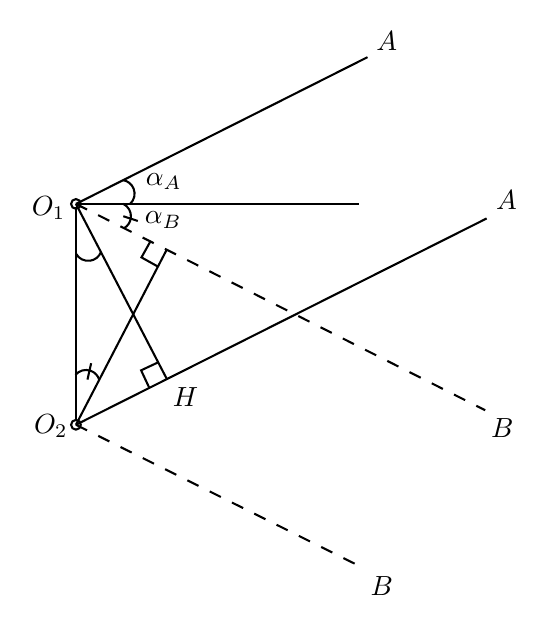
\begin{tikzpicture}[x=0.75pt,y=0.75pt,yscale=-1,xscale=1,scale=0.7]
%uncomment if require: \path (0,466); %set diagram left start at 0, and has height of 466

%Straight Lines [id:da9819586254374542] 
\draw    (100,152.52) -- (100,299.82) ;
\draw [shift={(100,302.17)}, rotate = 90] [color={rgb, 255:red, 0; green, 0; blue, 0 }  ][line width=0.75]      (0, 0) circle [x radius= 3.35, y radius= 3.35]   ;
\draw [shift={(100,150.17)}, rotate = 90] [color={rgb, 255:red, 0; green, 0; blue, 0 }  ][line width=0.75]      (0, 0) circle [x radius= 3.35, y radius= 3.35]   ;
%Straight Lines [id:da7435682220279671] 
\draw    (100,150.17) -- (294.67,150.17) ;
%Straight Lines [id:da28887576191566966] 
\draw    (100,150.17) -- (300.67,49.17) ;
%Straight Lines [id:da43527455840609197] 
\draw    (100,302.17) -- (382.67,160.17) ;
%Straight Lines [id:da04039868934755475] 
\draw  [dash pattern={on 4.5pt off 4.5pt}]  (100,150.17) -- (381.67,292.17) ;
%Straight Lines [id:da710611963130326] 
\draw  [dash pattern={on 4.5pt off 4.5pt}]  (100,302.17) -- (298.67,401.17) ;
%Straight Lines [id:da23804683123891368] 
\draw    (100,150.17) -- (162.63,270.78) ;
%Shape: Half Frame [id:dp9955568143034432] 
\draw   (144.86,264.71) -- (156.63,259.19) -- (156.63,259.19) -- (144.86,264.71) -- (150.37,276.48) -- (150.37,276.48) -- cycle ;
%Shape: Arc [id:dp08330355738741924] 
\draw  [draw opacity=0] (132.48,133.79) .. controls (135.64,134.33) and (138.45,136.46) .. (139.71,139.65) .. controls (141.21,143.43) and (140.1,147.6) .. (137.26,150.18) -- (130.89,143.14) -- cycle ; \draw   (132.48,133.79) .. controls (135.64,134.33) and (138.45,136.46) .. (139.71,139.65) .. controls (141.21,143.43) and (140.1,147.6) .. (137.26,150.18) ;
%Shape: Arc [id:dp6203513322329486] 
\draw  [draw opacity=0] (132.52,150.09) .. controls (136.03,151.79) and (138.26,155.56) .. (137.82,159.65) .. controls (137.49,162.73) and (135.73,165.3) .. (133.27,166.78) -- (128.39,158.64) -- cycle ; \draw   (132.52,150.09) .. controls (136.03,151.79) and (138.26,155.56) .. (137.82,159.65) .. controls (137.49,162.73) and (135.73,165.3) .. (133.27,166.78) ;
%Straight Lines [id:da6730799220969803] 
\draw    (132.58,158.63) -- (142.58,161.88) ;
%Shape: Arc [id:dp3410511987446969] 
\draw  [draw opacity=0] (117.12,183.57) .. controls (115.87,186.52) and (113.15,188.76) .. (109.75,189.25) .. controls (105.72,189.84) and (101.92,187.8) .. (100.07,184.43) -- (108.39,179.86) -- cycle ; \draw   (117.12,183.57) .. controls (115.87,186.52) and (113.15,188.76) .. (109.75,189.25) .. controls (105.72,189.84) and (101.92,187.8) .. (100.07,184.43) ;
%Straight Lines [id:da42548071910967367] 
\draw    (162.33,181.93) -- (100,302.17) ;
%Shape: Half Frame [id:dp49014282292792455] 
\draw   (145.11,186.96) -- (151.46,175.62) -- (151.46,175.62) -- (145.11,186.96) -- (156.45,193.31) -- (156.45,193.31) -- cycle ;
%Shape: Arc [id:dp5847002606176483] 
\draw  [draw opacity=0] (99.66,267.86) .. controls (102.15,264.86) and (106.35,263.6) .. (110.22,265.02) .. controls (113.12,266.09) and (115.19,268.42) .. (116.03,271.16) -- (106.95,273.93) -- cycle ; \draw   (99.66,267.86) .. controls (102.15,264.86) and (106.35,263.6) .. (110.22,265.02) .. controls (113.12,266.09) and (115.19,268.42) .. (116.03,271.16) ;
%Straight Lines [id:da962133525872563] 
\draw    (107.95,271.06) -- (110.47,259.8) ;

% Text Node
\draw (67.5,142.9) node [anchor=north west][inner sep=0.75pt]    {$O_{1}$};
% Text Node
\draw (69,292.9) node [anchor=north west][inner sep=0.75pt]    {$O_{2}$};
% Text Node
\draw (164.63,274.18) node [anchor=north west][inner sep=0.75pt]    {$H$};
% Text Node
\draw (304.67,29.57) node [anchor=north west][inner sep=0.75pt]    {$A$};
% Text Node
\draw (387,138.73) node [anchor=north west][inner sep=0.75pt]    {$A$};
% Text Node
\draw (383.67,295.57) node [anchor=north west][inner sep=0.75pt]    {$B$};
% Text Node
\draw (300.67,404.57) node [anchor=north west][inner sep=0.75pt]    {$B$};
% Text Node
\draw (146,127.23) node [anchor=north west][inner sep=0.75pt]    {$\alpha_{A}$};
% Text Node
\draw (145.26,153.58) node [anchor=north west][inner sep=0.75pt]    {$\alpha_{B}$};
\end{tikzpicture}
    \end{center}
    $A$ nhận được tín hiệu cực đại khi hai sóng từ $O_1$ và $O_2$ đến $A$ phải cùng pha hay độ lệch pha của hai sóng phải bằng $2\pi n$, với $n$ là một số nguyên. Độ lệch pha này bao gồm cả độ lệch pha ban đầu $\varphi$ và lệch pha do sóng từ thanh $O_2$ phải đi thêm một đoạn $O_2H = a \sin \alpha_A$ (với $a$ là khoảng cách giữa hai thanh). Vậy điều kiện tín hiệu cực đại cho $A$ là:
    \[\dfrac{2\pi a\sin \alpha_A }{\lambda} - \varphi = 2\pi n. \tag{1} \label{q.1.1}\]
    Tương tự, để cường độ tín hiệu đến $B$ đạt cực tiểu thì hai sóng phải ngược pha hay độ lệch pha của hai sóng phải bằng $(2n' + 1) \pi$, với $n'$ là một số nguyên.
    \[\dfrac{2\pi a\sin \alpha_B }{\lambda} - \varphi = (2n' + 1)\pi.  \tag{2} \label{q.1.2}\]
    Từ (\ref{q.1.1}) và (\ref{q.1.2}) suy ra:
    \[a \left( \sin\alpha_A - \sin\alpha_B \right) = \lambda \left(n - n' - \dfrac{1}{2} \right).\]
    Áp dụng công thức biến đổi $\sin$ và đặt $\alpha_A - \alpha_B = \beta$, ta được:
    \[2a \cos \left( \alpha_A - \dfrac{\beta}{2} \right) \sin \dfrac{\beta}{2} = \lambda \left( n - n' - \dfrac{1}{2} \right).\] 
    \[ \rt a = \dfrac{n - n' - \dfrac{1}{2}}{2\cos \left( \alpha_A - \dfrac{\beta}{2} \right) \sin \dfrac{\beta}{2}} \lambda. \tag{3} \label{q.1.3}\]
    Để $a$ đạt cực tiểu thì mẫu số đạt cực đại:
    \[\cos \left( \alpha_A - \dfrac{\beta}{2} \right) = 1 \rt \alpha_A = \dfrac{\beta}{2},\]
    và tử số phải cực tiểu:
    \[n - n' = 1.\]
    Thay vào (\ref{q.1.3}), ta có:
    \[a = \dfrac{\lambda}{4 \sin \dfrac{\beta}{2}},\quad \alpha_A = \dfrac{\beta}{2},\quad \alpha_B = - \dfrac{\beta}{2} ,\quad \varphi = \dfrac{\pi}{2} - 2\pi n.\]
    Vì không ảnh hưởng đến các tính chất vật lý nên ta có thể giả sử $n = 0$. Do đó, độ lệch pha giữa hai tín hiệu điện truyền cho hai thanh $\varphi = \dfrac{\pi}{2}$.\\
    \textbf{Nhận xét.} Pháp tuyến của mặt phẳng hai thanh tại $O_1$ là phân giác trong của góc giữa hai phương tới $A$ và $B$.
\item  Thay các thông số đề bài, ta tính được bước sóng $\lambda = \dfrac{c}{f} = 11,1 ~\mathrm{m}$, góc giữa hướng của $A$ và $B$: $\beta = 157^\circ - 72^\circ = 85^\circ$. Khoảng cách ngắn nhất giữa hai thanh là $a = 4,1 ~\mathrm{m}$.
\end{enumerate}

\begin{center}
    \bf Phần 2
\end{center}
\begin{center}

\tikzset{every picture/.style={line width=0.75pt}} %set default line width to 0.75pt        

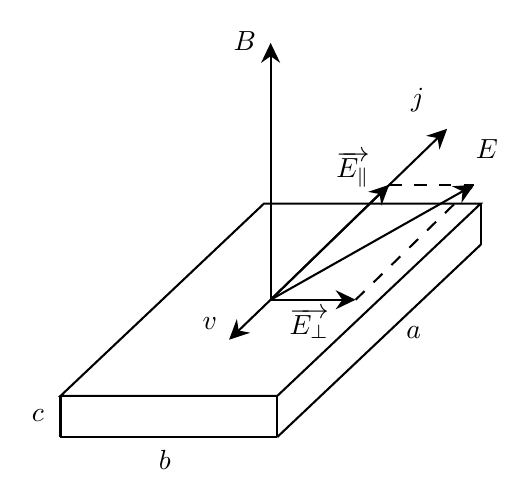
\begin{tikzpicture}[x=0.75pt,y=0.75pt,yscale=-1,xscale=1,scale=0.9]
%uncomment if require: \path (0,467); %set diagram left start at 0, and has height of 467

%Shape: Parallelogram [id:dp373425709308715] 
\draw   (292.95,191.67) -- (409,191.67) -- (300.05,294.67) -- (184,294.67) -- cycle ;
%Straight Lines [id:da08259287410986116] 
\draw    (184,294.67) -- (184,316.67) ;
%Straight Lines [id:da624429415382147] 
\draw    (184,316.67) -- (300.05,316.67) ;
%Straight Lines [id:da5856003144632871] 
\draw    (300.05,294.67) -- (300.05,316.67) ;
%Straight Lines [id:da6275847134856631] 
\draw    (409,213.67) -- (300.05,316.67) ;
%Straight Lines [id:da3859686385655472] 
\draw    (409,191.67) -- (409,199.67) -- (409,213.67) ;
%Straight Lines [id:da03239024585663475] 
\draw    (296.5,243.17) -- (296.5,108.67) ;
\draw [shift={(296.5,105.67)}, rotate = 450] [fill={rgb, 255:red, 0; green, 0; blue, 0 }  ][line width=0.08]  [draw opacity=0] (10.72,-5.15) -- (0,0) -- (10.72,5.15) -- (7.12,0) -- cycle    ;
%Straight Lines [id:da11775608008007676] 
\draw    (296.5,243.17) -- (388.84,153.75) ;
\draw [shift={(391,151.67)}, rotate = 495.92] [fill={rgb, 255:red, 0; green, 0; blue, 0 }  ][line width=0.08]  [draw opacity=0] (10.72,-5.15) -- (0,0) -- (10.72,5.15) -- (7.12,0) -- cycle    ;
%Straight Lines [id:da4041273396073155] 
\draw    (296.5,243.17) -- (357.8,183.71) ;
\draw [shift={(359.95,181.62)}, rotate = 495.87] [fill={rgb, 255:red, 0; green, 0; blue, 0 }  ][line width=0.08]  [draw opacity=0] (10.72,-5.15) -- (0,0) -- (10.72,5.15) -- (7.12,0) -- cycle    ;
%Straight Lines [id:da4069468675550836] 
\draw    (296.5,243.17) -- (339,243.17) ;
\draw [shift={(342,243.17)}, rotate = 180] [fill={rgb, 255:red, 0; green, 0; blue, 0 }  ][line width=0.08]  [draw opacity=0] (10.72,-5.15) -- (0,0) -- (10.72,5.15) -- (7.12,0) -- cycle    ;
%Straight Lines [id:da15993383163353347] 
\draw    (296.5,243.17) -- (276.43,262.49) ;
\draw [shift={(274.27,264.57)}, rotate = 316.09000000000003] [fill={rgb, 255:red, 0; green, 0; blue, 0 }  ][line width=0.08]  [draw opacity=0] (10.72,-5.15) -- (0,0) -- (10.72,5.15) -- (7.12,0) -- cycle    ;
%Straight Lines [id:da46530510829814986] 
\draw  [dash pattern={on 4.5pt off 4.5pt}]  (359.95,181.62) -- (405.45,181.62) ;
%Straight Lines [id:da49454551202265007] 
\draw  [dash pattern={on 4.5pt off 4.5pt}]  (342,243.17) -- (405.45,181.62) ;
%Straight Lines [id:da5869145777418041] 
\draw    (296.5,243.17) -- (402.84,183.09) ;
\draw [shift={(405.45,181.62)}, rotate = 510.54] [fill={rgb, 255:red, 0; green, 0; blue, 0 }  ][line width=0.08]  [draw opacity=0] (10.72,-5.15) -- (0,0) -- (10.72,5.15) -- (7.12,0) -- cycle    ;

% Text Node
\draw (330,162.07) node [anchor=north west][inner sep=0.75pt]    {$\overrightarrow{E_{\parallel}}$};
% Text Node
\draw (275,98.07) node [anchor=north west][inner sep=0.75pt]    {$\ot{B}$};
% Text Node
\draw (305,246.07) node [anchor=north west][inner sep=0.75pt]    {$\overrightarrow{E_{\perp}}$};
% Text Node
\draw (370,128.07) node [anchor=north west][inner sep=0.75pt]    {$\ot{j}$};
% Text Node
\draw (258.5,251.07) node [anchor=north west][inner sep=0.75pt]    {$\ot{v}$};
% Text Node
\draw (367.5,256.07) node [anchor=north west][inner sep=0.75pt]    {$a$};
% Text Node
\draw (235,322.07) node [anchor=north west][inner sep=0.75pt]    {$b$};
% Text Node
\draw (167,300.07) node [anchor=north west][inner sep=0.75pt]    {$c$};
% Text Node
\draw (404.67,155.9) node [anchor=north west][inner sep=0.75pt]    {$\ot{E}$};
\end{tikzpicture}
\end{center}
\begin{enumerate}[1)]
    \item Cường độ dòng điện trong thanh được tính bởi:
    \[I = jS = nev bc. \]
    Trong đó $j$ là mật độ dòng điện, $n$ là mật độ electron, $v$ là tốc độ electron, $S = bc$ là tiết diện của thanh. Ta suy ra:
    \[v = \dfrac{I}{nebc} = 25~\mathrm{m/s}. \]
    Điện trường trong thanh gồm hai thành phần vuông góc nhau: 
    \begin{itemize}
        \item Thành phần $E_\parallel$ song song với cạnh $a$ sinh ra dòng điện $I$:
    \[E_\parallel = \dfrac{v}{\mu} = 3,2~\mathrm{V/m}.\]
        \item Và thành phần $E_\perp$ sinh ra do lực Lorenz tác dụng electron làm cho các electron dồn về một phía (hiệu  ứng Hall):
    \[F_E = F_B \rt eE_\perp  = evB \rt E_\perp = vB = 2,5 ~\mathrm{V/m}.\]
    \end{itemize}
    
    Độ lớn của điện trường trong thanh:
    \[E = \sqrt{E_\parallel^2 + E_\perp^2} = 4,06 ~\mathrm{V/m}.\]
    \textbf{Lưu ý.} Vận tốc của electron ngược chiều dòng điện.
    \item Hiệu điện thế giữa hai điểm đối diện nhau trên hai mặt vuông góc với cạnh $b$ còn được gọi là hiệu điện thế Hall.
    \[U_H = E_\perp b = vBb = 25~\mathrm{mV}. \]
    \item Nếu dòng điện $I$ và từ trường $B$ đều là xoay chiều thì hiệu điện thế Hall thay đổi theo thời gian.
    \[U_H = vBb = \dfrac{IBb}{nebc} = \dfrac{I_0B_0}{nec} \sin \omega t \sin \omega \left( \omega t + \varphi \right).\]
    Vì 
    \[\sin \omega t \sin \omega \left( \omega t + \varphi \right) = \dfrac{1}{2} \left( \cos \varphi - \cos \left( 2\omega t + \varphi \right) \right)\]
    nên thành phần không đổi (DC) của $U_H$ là:
    \[U_{H0} = \dfrac{I_0B_0}{2nec} \cos \varphi.\]
    \item Hình dưới là sơ đồ mạch điện khả dĩ. Trong đó, $A$ là thiết bị điện cần đo công suất, $H$ là thanh có hiệu ứng Hall. Dòng điện qua thanh tỉ lệ với dòng điện qua $A$, cảm ứng từ $B$ tỉ lệ với hiệu điện thế đặt vào $A$. Đo $U_{H0}$, ta có một đại lượng tỉ lệ với công suất tiêu thụ của $A$.
    \begin{center}
    

\tikzset{every picture/.style={line width=0.75pt}} %set default line width to 0.75pt        

\begin{tikzpicture}[x=0.75pt,y=0.75pt,yscale=-1,xscale=1]
%uncomment if require: \path (0,378); %set diagram left start at 0, and has height of 378

%Shape: Right Angle [id:dp5818646696382868] 
\draw   (313,119.44) -- (435.5,119.44) -- (435.5,145.08) ;
%Flowchart: Process [id:dp628650293062013] 
\draw   (271.67,108.78) -- (312.33,108.78) -- (312.33,130.11) -- (271.67,130.11) -- cycle ;
%Shape: Inductor (Air Core) [id:dp26339175719770536] 
\draw   (242.17,221.94) -- (242.17,205.41) .. controls (237.55,205.41) and (233.8,202.12) .. (233.8,198.07) .. controls (233.8,194.01) and (237.55,190.72) .. (242.17,190.72) .. controls (237.55,190.72) and (233.8,187.43) .. (233.8,183.37) .. controls (233.8,179.32) and (237.55,176.03) .. (242.17,176.03) .. controls (237.55,176.03) and (233.8,172.74) .. (233.8,168.68) .. controls (233.8,164.63) and (237.55,161.33) .. (242.17,161.33) .. controls (237.55,161.33) and (233.8,158.04) .. (233.8,153.99) .. controls (233.8,149.93) and (237.55,146.64) .. (242.17,146.64) -- (242.17,130.11) ;
%Shape: Right Angle [id:dp42217384402675373] 
\draw   (242.17,130.11) -- (242.17,121.08) -- (271.67,121.08) ;
%Shape: Right Angle [id:dp8250782962105698] 
\draw   (367.17,224.58) -- (242.17,224.58) -- (242.17,221.94) ;
%Shape: Rectangle [id:dp3118917449720009] 
\draw   (368,214.83) -- (408,214.83) -- (408,234.08) -- (368,234.08) -- cycle ;
%Shape: Rectangle [id:dp2591240977513869] 
\draw   (422,146.83) -- (449.5,146.83) -- (449.5,196.08) -- (422,196.08) -- cycle ;
%Shape: Right Angle [id:dp7435516770236874] 
\draw   (436,196.58) -- (436,223.83) -- (408.5,223.83) ;
%Shape: Right Angle [id:dp5291623712489302] 
\draw   (422.56,223.67) -- (422.56,261.67) -- (201.89,261.67) ;
%Shape: Right Angle [id:dp1067855475193158] 
\draw   (201.89,261.67) -- (201.89,243.53) -- (208.73,243.53) ;
%Flowchart: Process [id:dp253784835356202] 
\draw   (209.33,233.33) -- (275.93,233.33) -- (275.93,253.93) -- (209.33,253.93) -- cycle ;
%Shape: Right Angle [id:dp37331800453169683] 
\draw   (339.87,224.2) -- (339.87,243.83) -- (276.37,243.83) ;
%Straight Lines [id:da9361994694141029] 
\draw    (339.47,119.47) -- (339.47,159.05) ;
\draw [shift={(339.47,161.4)}, rotate = 90] [color={rgb, 255:red, 0; green, 0; blue, 0 }  ][line width=0.75]      (0, 0) circle [x radius= 3.35, y radius= 3.35]   ;
%Straight Lines [id:da7608745159955392] 
\draw    (339.87,184.62) -- (339.87,224.2) ;
\draw [shift={(339.87,182.27)}, rotate = 90] [color={rgb, 255:red, 0; green, 0; blue, 0 }  ][line width=0.75]      (0, 0) circle [x radius= 3.35, y radius= 3.35]   ;
%Straight Lines [id:da6260889100847393] 
\draw    (220,187.53) -- (220,153.33) ;
\draw [shift={(220,150.33)}, rotate = 450] [fill={rgb, 255:red, 0; green, 0; blue, 0 }  ][line width=0.08]  [draw opacity=0] (10.72,-5.15) -- (0,0) -- (10.72,5.15) -- (7.12,0) -- cycle    ;
%Straight Lines [id:da9088167514605938] 
\draw    (216.43,243.42) -- (243.42,243.42) ;
\draw [shift={(246.42,243.42)}, rotate = 180] [fill={rgb, 255:red, 0; green, 0; blue, 0 }  ][line width=0.08]  [draw opacity=0] (10.72,-5.15) -- (0,0) -- (10.72,5.15) -- (7.12,0) -- cycle    ;

% Text Node
\draw (431,163.89) node [anchor=north west][inner sep=0.75pt]   [align=left] {A};
% Text Node
\draw (368.67,195.07) node [anchor=north west][inner sep=0.75pt]   [align=left] {Điện kế};
% Text Node
\draw (201.47,157.73) node [anchor=north west][inner sep=0.75pt]    {$\ot{B}$};
% Text Node
\draw (250.53,168.93) node [anchor=north west][inner sep=0.75pt]    {$L$};
% Text Node
\draw (250.67,236.32) node [anchor=north west][inner sep=0.75pt]    {$I$};
% Text Node
\draw (262.67,87.07) node [anchor=north west][inner sep=0.75pt]    {$R\gg \omega L$};
% Text Node
\draw (178,234.4) node [anchor=north west][inner sep=0.75pt]    {$H$};
\end{tikzpicture}

    \end{center}
\end{enumerate}
\end{loigiai}


\begin{vd}[Cáp đồng trục và vector Poynting]
Một cáp đồng trục rất dài (xem hình vẽ) mang dòng điện không đổi $I$ hướng lên trên dọc theo lõi dẫn điện bên trong và dòng điện dội lại $I$ hướng xuống dưới dọc theo vỏ dẫn điện bên ngoài. Mỗi lõi đều có chung mật độ điện trở dài (điện trở trên một đơn vị chiều dài) $\lambda$. Khoảng trống giữa lõi trụ và vỏ trụ là chân không.
   \begin{center}


\tikzset{every picture/.style={line width=0.75pt}} %set default line width to 0.75pt        

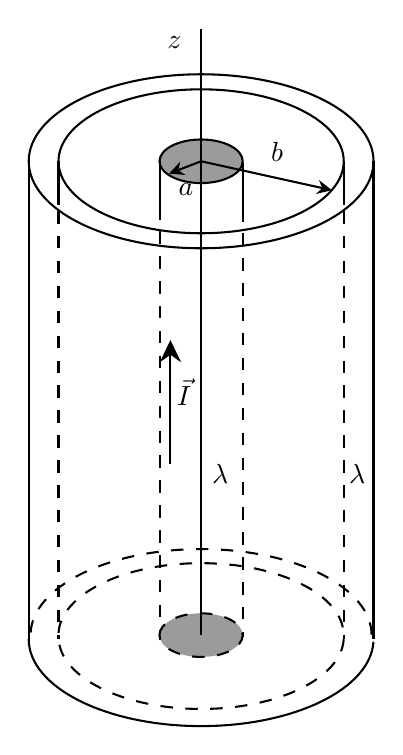
\begin{tikzpicture}[x=0.75pt,y=0.75pt,yscale=-1,xscale=1]
%uncomment if require: \path (0,506); %set diagram left start at 0, and has height of 506

%Shape: Ellipse [id:dp7387131786963701] 
\draw   (226.9,137.07) .. controls (226.9,117.92) and (257.66,102.4) .. (295.6,102.4) .. controls (333.55,102.4) and (364.31,117.92) .. (364.31,137.07) .. controls (364.31,156.22) and (333.55,171.74) .. (295.6,171.74) .. controls (257.66,171.74) and (226.9,156.22) .. (226.9,137.07) -- cycle ;
%Straight Lines [id:da44524678700877907] 
\draw  [dash pattern={on 4.5pt off 4.5pt}]  (226.9,137.07) -- (226.9,367.2) ;
%Straight Lines [id:da5045425062092759] 
\draw  [dash pattern={on 4.5pt off 4.5pt}]  (364.31,137.07) -- (364.31,367.2) ;
%Shape: Arc [id:dp9096024148344624] 
\draw  [draw opacity=0][dash pattern={on 4.5pt off 4.5pt}] (226.9,364.32) .. controls (228.01,345.66) and (258.33,330.7) .. (295.57,330.7) .. controls (333.52,330.7) and (364.28,346.22) .. (364.28,365.37) .. controls (364.28,365.4) and (364.28,365.43) .. (364.28,365.45) -- (295.57,365.37) -- cycle ; \draw  [dash pattern={on 4.5pt off 4.5pt}] (226.9,364.32) .. controls (228.01,345.66) and (258.33,330.7) .. (295.57,330.7) .. controls (333.52,330.7) and (364.28,346.22) .. (364.28,365.37) .. controls (364.28,365.4) and (364.28,365.43) .. (364.28,365.45) ;
%Shape: Arc [id:dp2738377078931662] 
\draw  [draw opacity=0][dash pattern={on 4.5pt off 4.5pt}] (364.3,367.33) .. controls (363.19,385.99) and (332.87,400.94) .. (295.63,400.94) .. controls (257.68,400.94) and (226.92,385.42) .. (226.92,366.27) .. controls (226.92,366.24) and (226.92,366.22) .. (226.92,366.19) -- (295.63,366.27) -- cycle ; \draw  [dash pattern={on 4.5pt off 4.5pt}] (364.3,367.33) .. controls (363.19,385.99) and (332.87,400.94) .. (295.63,400.94) .. controls (257.68,400.94) and (226.92,385.42) .. (226.92,366.27) .. controls (226.92,366.24) and (226.92,366.22) .. (226.92,366.19) ;
%Straight Lines [id:da9763316322078572] 
\draw  [dash pattern={on 4.5pt off 4.5pt}]  (275.7,170.8) -- (275.7,366.83) ;
%Straight Lines [id:da35128985625598075] 
\draw  [dash pattern={on 4.5pt off 4.5pt}]  (315.6,171.8) -- (315.6,366.15) ;
%Shape: Ellipse [id:dp7918229599786717] 
\draw  [fill={rgb, 255:red, 155; green, 155; blue, 155 }  ,fill opacity=1 ] (275.55,137.07) .. controls (275.55,131.27) and (284.53,126.57) .. (295.6,126.57) .. controls (306.68,126.57) and (315.65,131.27) .. (315.65,137.07) .. controls (315.65,142.87) and (306.68,147.57) .. (295.6,147.57) .. controls (284.53,147.57) and (275.55,142.87) .. (275.55,137.07) -- cycle ;
%Straight Lines [id:da15251740269356096] 
\draw    (275.7,137.07) -- (275.7,165.2) ;
%Straight Lines [id:da09211253848355194] 
\draw    (315.6,138.07) -- (315.6,166.2) ;
%Shape: Ellipse [id:dp761787885616863] 
\draw  [fill={rgb, 255:red, 155; green, 155; blue, 155 }  ,fill opacity=1 ][dash pattern={on 4.5pt off 4.5pt}] (275.52,365.37) .. controls (275.52,359.57) and (284.5,354.87) .. (295.57,354.87) .. controls (306.65,354.87) and (315.63,359.57) .. (315.63,365.37) .. controls (315.63,371.17) and (306.65,375.87) .. (295.57,375.87) .. controls (284.5,375.87) and (275.52,371.17) .. (275.52,365.37) -- cycle ;
%Straight Lines [id:da21889173081043856] 
\draw    (295.57,73.2) -- (295.57,365.37) ;
%Straight Lines [id:da3315018780674599] 
\draw    (282.93,141.93) -- (295.6,137.07) ;
\draw [shift={(280.13,143)}, rotate = 339.02] [fill={rgb, 255:red, 0; green, 0; blue, 0 }  ][line width=0.08]  [draw opacity=0] (7.14,-3.43) -- (0,0) -- (7.14,3.43) -- (4.74,0) -- cycle    ;
%Straight Lines [id:da5393246729054446] 
\draw    (355.69,150.35) -- (295.6,137.07) ;
\draw [shift={(358.62,151)}, rotate = 192.47] [fill={rgb, 255:red, 0; green, 0; blue, 0 }  ][line width=0.08]  [draw opacity=0] (7.14,-3.43) -- (0,0) -- (7.14,3.43) -- (4.74,0) -- cycle    ;
%Straight Lines [id:da3503244553627549] 
\draw    (280.82,226.2) -- (280.82,283.07) ;
\draw [shift={(280.82,223.2)}, rotate = 90] [fill={rgb, 255:red, 0; green, 0; blue, 0 }  ][line width=0.08]  [draw opacity=0] (10.72,-5.15) -- (0,0) -- (10.72,5.15) -- (7.12,0) -- cycle    ;
%Shape: Ellipse [id:dp41017552965576853] 
\draw   (212.54,137.07) .. controls (212.54,113.92) and (249.73,95.15) .. (295.6,95.15) .. controls (341.48,95.15) and (378.67,113.92) .. (378.67,137.07) .. controls (378.67,160.22) and (341.48,178.98) .. (295.6,178.98) .. controls (249.73,178.98) and (212.54,160.22) .. (212.54,137.07) -- cycle ;
%Straight Lines [id:da4132752834774358] 
\draw    (212.54,137.07) -- (212.54,367.2) ;
%Straight Lines [id:da8854408126227644] 
\draw    (378.67,137.07) -- (378.67,367.2) ;
%Shape: Arc [id:dp6298570830226897] 
\draw  [draw opacity=0][dash pattern={on 4.5pt off 4.5pt}] (213.46,364.11) .. controls (214.78,341.8) and (251.04,323.92) .. (295.57,323.92) .. controls (340.94,323.92) and (377.73,342.48) .. (377.73,365.37) .. controls (377.73,365.4) and (377.72,365.44) .. (377.72,365.47) -- (295.57,365.37) -- cycle ; \draw  [dash pattern={on 4.5pt off 4.5pt}] (213.46,364.11) .. controls (214.78,341.8) and (251.04,323.92) .. (295.57,323.92) .. controls (340.94,323.92) and (377.73,342.48) .. (377.73,365.37) .. controls (377.73,365.4) and (377.72,365.44) .. (377.72,365.47) ;
%Shape: Arc [id:dp21216290712255126] 
\draw  [draw opacity=0] (378.63,368.56) .. controls (377.29,391.12) and (340.63,409.2) .. (295.6,409.2) .. controls (249.73,409.2) and (212.54,390.44) .. (212.54,367.29) .. controls (212.54,367.26) and (212.54,367.22) .. (212.54,367.19) -- (295.6,367.29) -- cycle ; \draw   (378.63,368.56) .. controls (377.29,391.12) and (340.63,409.2) .. (295.6,409.2) .. controls (249.73,409.2) and (212.54,390.44) .. (212.54,367.29) .. controls (212.54,367.26) and (212.54,367.22) .. (212.54,367.19) ;
%Straight Lines [id:da32646367186187697] 
\draw    (226.9,137.07) -- (226.9,158.2) ;
%Straight Lines [id:da7218847112054345] 
\draw    (364.31,137.07) -- (364.31,158.2) ;


% Text Node
\draw (277.84,75.4) node [anchor=north west][inner sep=0.75pt]    {$z$};
% Text Node
\draw (282.39,240.4) node [anchor=north west][inner sep=0.75pt]    {$\vec{I}$};
% Text Node
\draw (283.3,146.4) node [anchor=north west][inner sep=0.75pt]    {$a$};
% Text Node
\draw (327.89,126.4) node [anchor=north west][inner sep=0.75pt]    {$b$};
% Text Node
\draw (299.45,281.4) node [anchor=north west][inner sep=0.75pt]    {$\lambda $};
% Text Node
\draw (365.43,281.4) node [anchor=north west][inner sep=0.75pt]    {$\lambda $};


\end{tikzpicture}
\end{center}

Bán kính của lõi trụ trong là $a$ và bán kính lõi trụ ngoài là $b$. Trong bài toán này ta sẽ sử dụng hệ tọa độ trụ, $\rho, \varphi, z$. Trong hệ tọa độ đó ta có:
   $$\nabla^2 \phi = \frac{1}{\rho}\frac{\partial}{\partial\rho}\left(\rho\frac{\partial\phi}{\partial\rho}\right) + \frac{1}{\rho^2} \frac{\partial^2 \phi}{\partial \varphi^2} + \frac{\partial^2 \phi}{\partial z^2}.$$
 \begin{enumerate}[1)] 
    \item Tính điện thế  và cường độ điện trường trong vùng $a\leq \rho \leq b$. Công nhận rằng $E_{\rho}(\rho, \varphi, 0) = 0$.
   \item Tính từ trường trong vùng $a \leq \rho \leq b$.
   \item Tính vector Poynting trong vùng $a\leq \rho \leq b$ và tích phân nó trên toàn bộ bề mặt của vùng thể tích được giới hạn bởi $\rho =a,\, \rho = b,$ và $-l/2 \leq z \leq l/2$. Bình luận về ý nghĩa vật lý của kết quả thu được.
  \end{enumerate}


\end{vd}

\begin{loigiai}
  \begin{enumerate}[1)]
      \item Chúng ta có phương trình Laplace ở trong hệ tọa độ trụ:
  $$\phi (\rho, z) = (\alpha z +\beta)\ln  \left(\frac{\rho}{\rho_0}\right).$$
Từ điều kiện biên:
  $$\phi(\rho,0) = 0 \rt  \beta=0.$$
   $$\rt  \phi(\rho, z) = \alpha z \ln  \left(\frac{\rho}{\rho_0}\right).$$
        \begin{center}


\tikzset{every picture/.style={line width=0.75pt}} %set default line width to 0.75pt        

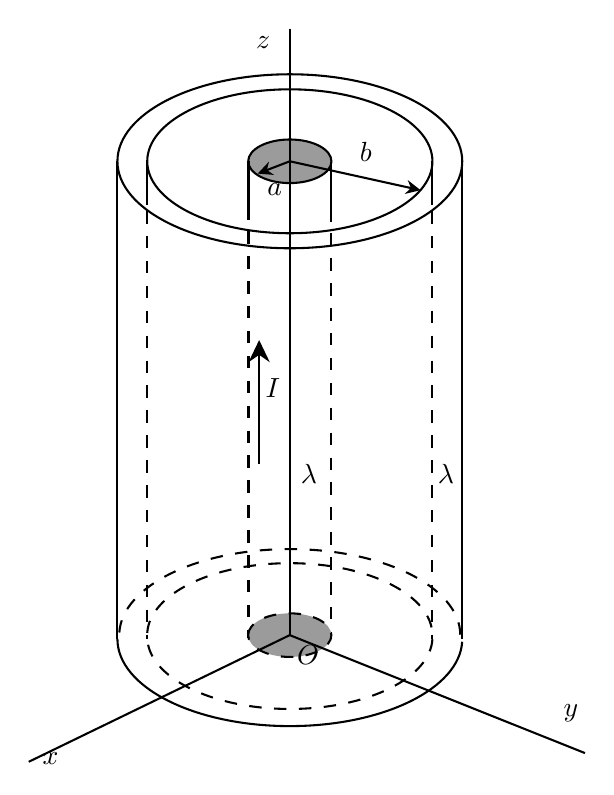
\begin{tikzpicture}[x=0.75pt,y=0.75pt,yscale=-1,xscale=1]
%uncomment if require: \path (0,506); %set diagram left start at 0, and has height of 506

%Shape: Ellipse [id:dp43219690364158425] 
\draw   (226.9,137.07) .. controls (226.9,117.92) and (257.66,102.4) .. (295.6,102.4) .. controls (333.55,102.4) and (364.31,117.92) .. (364.31,137.07) .. controls (364.31,156.22) and (333.55,171.74) .. (295.6,171.74) .. controls (257.66,171.74) and (226.9,156.22) .. (226.9,137.07) -- cycle ;
%Straight Lines [id:da8403669513412004] 
\draw  [dash pattern={on 4.5pt off 4.5pt}]  (226.9,137.07) -- (226.9,367.2) ;
%Straight Lines [id:da19439143327647157] 
\draw  [dash pattern={on 4.5pt off 4.5pt}]  (364.31,137.07) -- (364.31,367.2) ;
%Shape: Arc [id:dp24060319153376497] 
\draw  [draw opacity=0][dash pattern={on 4.5pt off 4.5pt}] (226.9,364.32) .. controls (228.01,345.66) and (258.33,330.7) .. (295.57,330.7) .. controls (333.52,330.7) and (364.28,346.22) .. (364.28,365.37) .. controls (364.28,365.4) and (364.28,365.43) .. (364.28,365.45) -- (295.57,365.37) -- cycle ; \draw  [dash pattern={on 4.5pt off 4.5pt}] (226.9,364.32) .. controls (228.01,345.66) and (258.33,330.7) .. (295.57,330.7) .. controls (333.52,330.7) and (364.28,346.22) .. (364.28,365.37) .. controls (364.28,365.4) and (364.28,365.43) .. (364.28,365.45) ;
%Shape: Arc [id:dp09179080796471828] 
\draw  [draw opacity=0][dash pattern={on 4.5pt off 4.5pt}] (364.3,367.33) .. controls (363.19,385.99) and (332.87,400.94) .. (295.63,400.94) .. controls (257.68,400.94) and (226.92,385.42) .. (226.92,366.27) .. controls (226.92,366.24) and (226.92,366.22) .. (226.92,366.19) -- (295.63,366.27) -- cycle ; \draw  [dash pattern={on 4.5pt off 4.5pt}] (364.3,367.33) .. controls (363.19,385.99) and (332.87,400.94) .. (295.63,400.94) .. controls (257.68,400.94) and (226.92,385.42) .. (226.92,366.27) .. controls (226.92,366.24) and (226.92,366.22) .. (226.92,366.19) ;
%Straight Lines [id:da49407652980227357] 
\draw  [dash pattern={on 4.5pt off 4.5pt}]  (275.7,170.8) -- (275.7,366.83) ;
%Straight Lines [id:da5608963847962924] 
\draw  [dash pattern={on 4.5pt off 4.5pt}]  (315.6,171.8) -- (315.6,366.15) ;
%Shape: Ellipse [id:dp7172021001895048] 
\draw  [fill={rgb, 255:red, 155; green, 155; blue, 155 }  ,fill opacity=1 ] (275.55,137.07) .. controls (275.55,131.27) and (284.53,126.57) .. (295.6,126.57) .. controls (306.68,126.57) and (315.65,131.27) .. (315.65,137.07) .. controls (315.65,142.87) and (306.68,147.57) .. (295.6,147.57) .. controls (284.53,147.57) and (275.55,142.87) .. (275.55,137.07) -- cycle ;
%Straight Lines [id:da3681511162782529] 
\draw    (275.7,137.07) -- (275.7,165.2) ;
%Straight Lines [id:da2163405263705387] 
\draw    (315.6,138.07) -- (315.6,166.2) ;
%Shape: Ellipse [id:dp8856875355730747] 
\draw  [fill={rgb, 255:red, 155; green, 155; blue, 155 }  ,fill opacity=1 ][dash pattern={on 4.5pt off 4.5pt}] (275.52,365.37) .. controls (275.52,359.57) and (284.5,354.87) .. (295.57,354.87) .. controls (306.65,354.87) and (315.63,359.57) .. (315.63,365.37) .. controls (315.63,371.17) and (306.65,375.87) .. (295.57,375.87) .. controls (284.5,375.87) and (275.52,371.17) .. (275.52,365.37) -- cycle ;
%Straight Lines [id:da10132036180260595] 
\draw    (295.57,73.2) -- (295.57,365.37) ;
%Straight Lines [id:da1033116435839283] 
\draw    (282.93,141.93) -- (295.6,137.07) ;
\draw [shift={(280.13,143)}, rotate = 339.02] [fill={rgb, 255:red, 0; green, 0; blue, 0 }  ][line width=0.08]  [draw opacity=0] (7.14,-3.43) -- (0,0) -- (7.14,3.43) -- (4.74,0) -- cycle    ;
%Straight Lines [id:da9175999059322228] 
\draw    (355.69,150.35) -- (295.6,137.07) ;
\draw [shift={(358.62,151)}, rotate = 192.47] [fill={rgb, 255:red, 0; green, 0; blue, 0 }  ][line width=0.08]  [draw opacity=0] (7.14,-3.43) -- (0,0) -- (7.14,3.43) -- (4.74,0) -- cycle    ;
%Straight Lines [id:da7414005162889266] 
\draw    (280.82,226.2) -- (280.82,283.07) ;
\draw [shift={(280.82,223.2)}, rotate = 90] [fill={rgb, 255:red, 0; green, 0; blue, 0 }  ][line width=0.08]  [draw opacity=0] (10.72,-5.15) -- (0,0) -- (10.72,5.15) -- (7.12,0) -- cycle    ;
%Shape: Ellipse [id:dp8956042166933398] 
\draw   (212.54,137.07) .. controls (212.54,113.92) and (249.73,95.15) .. (295.6,95.15) .. controls (341.48,95.15) and (378.67,113.92) .. (378.67,137.07) .. controls (378.67,160.22) and (341.48,178.98) .. (295.6,178.98) .. controls (249.73,178.98) and (212.54,160.22) .. (212.54,137.07) -- cycle ;
%Straight Lines [id:da49921180646613394] 
\draw    (212.54,137.07) -- (212.54,367.2) ;
%Straight Lines [id:da10822099505113725] 
\draw    (378.67,137.07) -- (378.67,367.2) ;
%Shape: Arc [id:dp6899138488334191] 
\draw  [draw opacity=0][dash pattern={on 4.5pt off 4.5pt}] (213.46,364.11) .. controls (214.78,341.8) and (251.04,323.92) .. (295.57,323.92) .. controls (340.94,323.92) and (377.73,342.48) .. (377.73,365.37) .. controls (377.73,365.4) and (377.72,365.44) .. (377.72,365.47) -- (295.57,365.37) -- cycle ; \draw  [dash pattern={on 4.5pt off 4.5pt}] (213.46,364.11) .. controls (214.78,341.8) and (251.04,323.92) .. (295.57,323.92) .. controls (340.94,323.92) and (377.73,342.48) .. (377.73,365.37) .. controls (377.73,365.4) and (377.72,365.44) .. (377.72,365.47) ;
%Shape: Arc [id:dp7467674110195988] 
\draw  [draw opacity=0] (378.63,368.56) .. controls (377.29,391.12) and (340.63,409.2) .. (295.6,409.2) .. controls (249.73,409.2) and (212.54,390.44) .. (212.54,367.29) .. controls (212.54,367.26) and (212.54,367.22) .. (212.54,367.19) -- (295.6,367.29) -- cycle ; \draw   (378.63,368.56) .. controls (377.29,391.12) and (340.63,409.2) .. (295.6,409.2) .. controls (249.73,409.2) and (212.54,390.44) .. (212.54,367.29) .. controls (212.54,367.26) and (212.54,367.22) .. (212.54,367.19) ;
%Straight Lines [id:da2674227113743717] 
\draw    (226.9,137.07) -- (226.9,158.2) ;
%Straight Lines [id:da8335025525773812] 
\draw    (364.31,137.07) -- (364.31,158.2) ;
%Straight Lines [id:da22805806038371035] 
\draw    (169.8,426.4) -- (295.57,365.37) ;
%Straight Lines [id:da03015767444311246] 
\draw    (437.8,422.2) -- (295.57,365.37) ;


% Text Node
\draw (277.84,75.4) node [anchor=north west][inner sep=0.75pt]    {$z$};
% Text Node
\draw (282.39,240.4) node [anchor=north west][inner sep=0.75pt]    {$\ot{I}$};
% Text Node
\draw (283.3,146.4) node [anchor=north west][inner sep=0.75pt]    {$a$};
% Text Node
\draw (327.89,126.4) node [anchor=north west][inner sep=0.75pt]    {$b$};
% Text Node
\draw (299.45,281.4) node [anchor=north west][inner sep=0.75pt]    {$\lambda $};
% Text Node
\draw (365.43,281.4) node [anchor=north west][inner sep=0.75pt]    {$\lambda $};
% Text Node
\draw (175,420.4) node [anchor=north west][inner sep=0.75pt]    {$x$};
% Text Node
\draw (426,397.4) node [anchor=north west][inner sep=0.75pt]    {$y$};
% Text Node
\draw (297.57,368.77) node [anchor=north west][inner sep=0.75pt]    {$O$};


\end{tikzpicture}
\end{center}

Tích phân độ sụt thế dọc theo cáp điện (xem hình vẽ), ta thu được:
\begin{align*}
    -I\lambda z &= \phi(a,z) - \phi(a,0),\\
    I\lambda z &= \phi(b,z) - \phi(b,0).
\end{align*}
Và do đó:
 $$ a=- \frac {2I\lambda}{\ln(a/b)}, \quad \rho_0 = \sqrt{ab},$$
ta thu được kết quả:
  $$\phi(\rho, z)=-I \lambda z \frac{\ln \left[\rho^{2} /(a b)\right]}{\ln (a / b)}=\left\{ \begin{array}{ll}
-I \lambda z, & \rho=a \\
I \lambda z, & \rho=b
\end{array} \right. .$$
Điện trường trong vùng đó là:
  $$\ot{E}=-\nabla \phi=-\frac{\partial \phi}{\partial \rho} \ot{e_{\rho}}-\frac{\partial \phi}{\partial z} \hat{{z}}=\frac{2 I \lambda z}{\rho \ln (a / b)} \ot{e_{\rho}}+\frac{I \lambda \ln \left[\rho^{2} /(a b)\right]}{\ln (a / b)} \hat{{z}} .$$
  \item Từ trường trong vùng $a<\rho<b$ có thể được tính từ các phương trình:
  \begin{align*}
      &\oint \ot{H}_{\varphi} \cdot \dd \ot{l} = \frac{4 \pi}{c} I\\
     &\rt  2 \pi \rho H_{\varphi} = \frac{4 \pi}{c} I\\
     &\rt  \ot{H} = H_{\varphi} \ot{e}_{\varphi}=\frac{2 I}{c \rho} \ot{e}_{\varphi}.
  \end{align*}
    \item Vector Poynting là:
       $$\ot{S} = \dfrac{c}{4\pi}(\ot{E}\times \ot{H}).$$
Chuyển $\ot{E}$ về hệ tọa độ Descartes, ta có:
\begin{align*}
    E_x &= E_{\rho}\cos\varphi - E_{\varphi}\sin\varphi,\\
    E_y &= E_{\rho}\sin\varphi + E_{\varphi}\cos\phi, \\
    E_z &= E_z.
\end{align*}

Phép đổi tương tự cũng được áp dụng cho $\ot{H}$, do đó ta thu được:
\begin{align*}
    {\ot { E }} \times \ot{H} &= \left|\begin{array}{ccc}
\hat{{x}} & \hat{{y}} & \hat{{z}} \\
E_{\rho} \cos \varphi & E_{\rho} \sin \varphi & E_{z} \\
-H_{\varphi} \sin \varphi & H_{\varphi} \cos \varphi & 0
\end{array}\right|\\
    &= -E_{z} H_{\varphi} \cos \varphi \hat{{x}}-E_{z} H_{\varphi} \sin \varphi \hat{{y}}+E_{\rho} H_{\varphi} \hat{{z}}\\
    &= -E_{z} H_{\varphi} \ot{e}_{\rho}+E_{\rho} H_{\varphi} \hat{{z}}.
\end{align*}
Nên:
\begin{align*}
    \ot{S} &= -\frac{c}{4 \pi} \frac{I \lambda \ln \left[\rho^{2} /(a b)\right]}{\ln (a / b)} \frac{2 I}{c \rho} \ot{e}_{\rho}+\frac{c}{4 \pi} \frac{2 I \lambda z}{\rho \ln (a / b)} \frac{2 I}{c \rho} \hat{{z}}\\
    &= -\frac{I^{2} \lambda \ln \left[\rho^{2} /(a b)\right]}{2 \pi \rho \ln (a / b)]} \ot{e}_{\rho}+\frac{I^{2} \lambda z}{\pi \rho^{2} \ln (a / b)} \hat{{z}}.
\end{align*}

Bây giờ ta tính dòng năng lượng $F^i$ và $F^o$ đi vào lõi dây dẫn trong và vỏ bên ngoài:
    $$F^{\mathrm{i}}=\int_{A} \ot{S} \cdot \dd \ot{A}=\frac{I^{2} \lambda \ln (a / b)}{2 \pi a \ln (a / b)} 2 \pi a \cdot l=I^{2} \lambda l=I^{2} R,$$
    $$F^{o}=\int_{A} \ot{S} \cdot \dd \ot{A}=\frac{I^{2} \lambda \ln (a / b)}{2 \pi b \ln (a / b)} 2 \pi b \cdot l=I^{2} \lambda l=I^{2} R ,$$
ở đây R là điện trở của một đoạn dây dẫn dài $l$ của cả lõi dây và vỏ dây. Tổng dòng năng lượng đi vào dây dẫn là $F=F^i + F^o = 2I^2 R$, tương ứng với nhiệt lượng Joule tỏa ra từ điện trở. Vì vùng chân không giữa vỏ dây và lõi dây không có dòng điện chạy qua và hệ đang ở trạng thái ổn định nên định luật Poynting được áp dụng:
      $$\nabla \cdot \ot{S} = 0. $$
Tổng dòng năng lượng vào và ra phải bằng không. Cho nên phải có một dòng năng lượng âm $F_e$ đi vào vùng thể tích này qua hai đầu dây để thỏa mãn định luật Poynting. Do đó:
    \begin{align*}
        F^e &= \int_{A} S_z {\hat{z}} \cdot \dd \ot{A} = \left(\frac{l}{2} - \frac{-l}{2}\right) \int_{a}^{b} \frac{I^2 \lambda}{\pi\rho^2 \ln (a/b)} 2 \pi\rho \dd \rho\\
        &= \frac{2\pi I^2 \lambda l \text{ln}(b/a)}{\pi \text{ln}(a/b)} = -2I^2 \lambda l = -2I^2 R.
    \end{align*}
kết quả thu được giống như ta dự đoán từ đầu.
\end{enumerate}
\end{loigiai}


\begin{vd}[Năng lượng ở đâu?]
%USAPhO 2015
Bài này đưa ra ba tình huống để chuyển hóa năng lượng vào một vùng không gian của trường điện từ. Trong tình huống đầu tiên, năng lượng đó được tích trữ dưới dạng động năng của một vật mang điện, ở tình huống thứ hai và thứ ba, năng lượng được tích trữ trong điện trường hoặc từ trường.\\
Nói chúng, bất cứ khi nào một điện trường và một từ trường không cùng phương với nhau, thì năng lượng đều được chuyển hóa; ví dụ, nguyên tắc này là lí do mà bức xạ điện từ có chuyển hóa năng lượng. Năng lượng chuyển hóa trên một đơn vị diện tích được cho bởi \textit{vector Poynting}:
$$\ot{S}=\dfrac{1}{\mu_0}\ot{E}\times\ot{B}.$$
Trong mỗi phần của bài này, phần nhỏ cuối cùng yêu cầu xác minh xem tốc độ chuyển hóa năng lượng có phù hợp với biểu thức của vector Poynting hay không. Do đó, không nên sử dụng biểu thức vector Poynting trước các phần nhỏ cuối cùng đó!
\begin{enumerate}[1)]
    \item Một thanh hình trụ dài cách điện có bán kính $R$ và có mật độ điện tích khối $\rho$. Một điện trường ngoài đều $E$ hướng dọc theo trục của hình trụ. Thanh chuyển động dọc theo trục của nó với tốc độ $v$.
    \begin{enumerate}[a)]
        \item Công suất trên một đơn vị chiều dài $\mathcal{P}$ đã truyền cho thanh là bao nhiêu?
        \item Từ trường $B$ tại bề mặt của thanh là bao nhiêu? Hãy vẽ hướng của từ trường trên sơ đồ.
        \item Tính toán vector Poynting. vẽ hướng của nó trên sơ đồ, và xác minh rằng nó phù hợp với tốc độ truyền năng lượng.
    \end{enumerate}
    \item Một tụ điện phẳng song song gồm hai đĩa có bán kính $R$ cách nhau một khoảng $d\ll R$. Tụ được tích điện $Q$ bởi một dòng điện nhỏ không đổi $I$.
    \begin{enumerate}[a)]
        \item Tìm công suất $P$ đã cung cấp cho tụ?
        \item Từ trường $B$ ở giữa hai bản tụ là bao nhiêu? Vẽ hướng của nó trên sơ đồ? (Bỏ qua các hiệu ứng dịch chuyển trong điện trường của các tính toán ở phần này).
        \item Hãy tính toán vector Poynting, vẽ hướng của nó ở trên sơ đồ, và xác minh rằng liệu nó có phù hợp với tốc độ chuyển hóa năng lượng hay không?
    \end{enumerate}
    \item Một ống solenoid có bán kính $R$ có $\mathcal{N}$ vòng dây trên một đơn vị chiều dài. Ống có dòng điện $I$ chạy qua, và dòng điện này được tăng lên với tốc độ nhỏ không đổi $\dfrac{\dd I}{\dd t}$.
    \begin{enumerate}[a)]
        \item Tìm công suất trên một đơn vị chiều dài $\mathcal{P}$ đã cung cấp cho ống solenoid.
        \item Hãy tìm điện trường $E$ ở bên trong ống solenoid? Vẽ hướng của nó trên sơ đồ.
        \item Tính toán vectore Poynting, vẽ hướng của nó trên sơ đồ, và xác minh tính phù hợp của nó với tốc độ chuyển hóa năng lượng.
    \end{enumerate}
\end{enumerate}
\end{vd}
\begin{loigiai}
\begin{enumerate}[1)]
    \item
    \begin{enumerate}[a)]
        \item Phần thanh có chiều dài $l$ có điện tích $q=\pi R^2 l \rho$, chịu lực tác dụng $F=qE$ và công suất truyền cho nó là $P=Fv$. Kết hợp các phương trình trên:
        $$ P=\pi R^2 l\rho Ev, \ \mathcal{P}=\pi R^2\rho Ev.$$
        \item Phần tử thanh dài $l$ sẽ chuyển động qua một điện trường trong khoảng thời gian $t=\dfrac{l}{v}$, do đó dòng điện trong thanh là :
        $$I=\dfrac{q}{t}=\pi R^2 \rho v.$$
        Áp dụng định luật Ampere cho vòng dây bán kính $R$,
        $$
\begin{aligned}
\oint \mathbf{B} \cdot \dd \mathbf{l} &=\mu_{0} I_{e n c}, \\
\rt 2 \pi R B=\mu_{0} \pi R^{2} \rho v & \Rightarrow \quad B=\frac{1}{2} \mu_{0} R \rho v.
\end{aligned}
$$
Từ trường có dạng hình tròn theo quy tắc bàn tay phải.
\item Từ trường và điện trường vuông góc nên vector Poynting có dạng:
$$S=\dfrac{1}{\mu_0}EB=\dfrac{1}{2}R\rho v E.$$
Áp dụng nhanh quy tắc bàn tay phải, ta thấy rằng vector này hướng vào trong theo phương bán kính của hình trụ, như ta dự đoán. Hình trụ có diện tích trên một đơn vị chiều dài là $2\pi R$, do đó công suất chuyển hóa năng lượng trên một đơn vị chiều dài là:
$$\mathcal{P}=2\pi R S=\pi R^2 \rho vE,$$
giống với kết quả của phần trước.
\end{enumerate}
\item \begin{enumerate}[a)]
    \item Điện dung của bản tụ song song được cho bởi công thức:
    $$C=\dfrac{\varepsilon \pi R^2}{d}.$$
    Điện thế trên bản tụ là:
    $$V=\dfrac{Q}{C}=\dfrac{Qd}{\varepsilon_0\pi R^2},$$
    và công suất là:
    $$P=IV=\dfrac{IQd}{\varepsilon_0\pi R^2}.$$
    Thay vào đó, ta có thể chọn áp dụng công thức cho mật độ khối của năng lượng:
    $$\mathcal{U}=\dfrac{1}{2}\varepsilon_0E^2.$$
    \item Xét một vòng Amperian bao quanh cạnh của tụ điện và dùng một mặt Gauss xuyên qua tâm của tụ điện. Điện trường vuông góc với mặt Gauss và có độ lớn:
    $$E=\dfrac{V}{d}=\dfrac{Q}{\varepsilon_0\pi R^2}.$$
    Điện thông đi qua mặt Gauss là:
    $$\phi_E = \pi R^2 E=\dfrac{Q}{\varepsilon_0}.$$
    Công thức này cũng có thể được xác định bằng cách trực tiếp sử dụng định luật Gauss và các phép đối xứng phù hợp. Không có dòng điện đi qua mặt phẳng, nên theo định lý Ampere:
     $$
\begin{aligned}
\oint \mathbf{B} \cdot \dd \mathbf{l} &=\mu_{0} \varepsilon_0 \dfrac{\dd \phi_E}{\dd t}, \\
\rt 2 \pi R B=\mu_{0} \dfrac{\dd Q}{\dd t} & \Rightarrow \quad B=\dfrac{\mu_0 I}{2\pi R}.
\end{aligned}
$$
Từ trường có dạng hình tròn như quy tắc bàn tay phải.\\
Lưu ý rằng thay vào đó, ta có thể sử dụng mặt Gauss cong để tránh tâm của tụ điện và tránh giao cắt với các dây tích điện! Trong trường hợp đó ta có thể làm trực tiếp:
$$\oint \mathbf{B} \cdot \dd \mathbf{l}=\mu_0 I,$$
và việc tính toán vẫn được tiến hành như trước.
\item Điện trường và từ trường vuông góc với nhau, do đó ta lại có:
$$S=\dfrac{1}{\mu_0}EB=\dfrac{IQ}{2\varepsilon_0\pi ^2R^3}.$$
Ứng dụng nhanh quy tắc bàn tay phải ta thấy rằng vector này hướng vào bên trong, dọc theo cạnh của tụ điện. Diện tích của vùng này là $2\pi R d$, do đó công suất được truyền là:
$$P=2\pi R\dd S=\dfrac{IQd}{\varepsilon_0\pi R^2},$$
phù hợp với kết quả trước đó.
\end{enumerate}
\item 
\begin{enumerate}[a)]
    \item Giả sử rằng cuộn dây solenoid có chiều dài $l$. Độ tự cảm là:
    $$L=\mu_0\mathcal{N}^2\pi R^2 l.$$
    Ta có thể trích dẫn trực tiếp công thức nào, hoặc suy ra bằng cách sau. Giả sử có một vòng Amperian có độ dài $d$ giao với ống solenoid. Vòng này bao quanh $\mathcal{N}d$ vòng dây, do đó theo định lý Ampere (nhớ rằng từ trường chỉ tồn tại phía bên trong ống solenoid):
    $$
\begin{aligned}
\oint \mathbf{B} \cdot \dd \mathbf{l} &=\mu_{0} I_{c n c}, \\
\rt B d=\mu_{0} \mathcal{N} \dd I & \Rightarrow B=\mu_{0} \mathcal{N} I.
\end{aligned}
$$
Có $\mathcal{N}l$ vòng dây, do đó tổng điện thông là:
$$\Phi =\mathcal{N}l B\pi R^2=\mu_0\mathcal{N}^2I\pi R^2 l,$$
và lại có $\Phi=LI$ nên:
$$L=\mu_0\mathcal{N}^2\pi R^2l,$$
như đã có ở trên.\\
Do đó, điện áp trên cuộn cảm là:
$$V=L\dfrac{\dd I}{\dd t}=\mu_0\mathcal{N}^2\pi R^2l\dfrac{\dd I}{\dd t}.$$
Và công suất truyền tải là:
$$P=IV=\mu_0\mathcal{N}^2\pi R^2l I\dfrac{\dd I}{\dd t},$$
hoặc, chia cho $l$:
$$\mathcal{P}=\mu_0\mathcal{N}^2\pi R^2I\dfrac{\dd I}{\dd t}.$$
Thay vào đó, ta có thể chọn áp dụng cho mật độ khối năng lượng:
$$\mathcal{U}=\dfrac{1}{2\mu_0}B^2.$$
\item Hãy xét một vòng Amperian ở ngay bên trong bề mặt của ống solenoid. Như ở trên, điện trường đi qua vòng này là $B=\mu_0\mathcal{N}I$, do đó:
$$
\begin{gathered}
\oint \mathbf{E} \cdot \dd l =\dfrac{\dd \phi_{B}}{\dd t}, \\
\rt 2 \pi R E=\mu_{0} \mathcal{N} \pi R^{2} \dfrac{\dd I}{d t} \Rightarrow E=\dfrac{1}{2} \mu_{0} \mathcal{N} R \dfrac{\dd I}{\dd t}.
\end{gathered}
$$
Điện trường có dạng hình tròn dựa theo định luật Lenz và quy tắc bàn tay phải.
\item Điện trường và từ trường vuông góc, nên một lần nữa ta có:
$$S=\dfrac{1}{\mu_0}EB=\dfrac{1}{2}\mu_0 \mathcal{N}^2 RI\dfrac{\dd I}{\dd t}.$$
Ứng dụng nhanh quy tắc bàn tay phải, ta thấy rằng vector Poynting hướng vào trong phía trục của ống solenoid. Diện tích trên một đơn vị chiều dài là $2\pi R$, do đó công suất trên một đơn vị chiều dài là;
$$\mathcal{P=2\pi RS}=\mu_0\mathcal{N}^2\pi R^2I\dfrac{\dd I}{\dd t},$$
phù hợp với các kết quả trước đó.
\end{enumerate}
\end{enumerate}
\end{loigiai}
